% NPMP, skupina 24
% Avtor: Žan Roštan

\graphicspath{{Skupina24/img/}}

\title{Vpliv napak vrat CNOT na učinkovitost očiščevanja Bellovih parov}
\author{Žan Roštan}
\maketitle

\abstract{V seminarski nalogi sem preveril, pri katerih začetnih zvestobah Bellovih parov in stopnjah šuma na vratih CNOT en krog očiščevanja BBPSSW še poveča zvestobo. V Qiskit Aer sem simuliral štiri kubite z gostotnimi matrikami in primerjal idealno izvedbo z izvedbo, kjer po obeh očiščevalnih vratih CNOT deluje depolarizacijski kanal. Za devet začetnih zvestob in deset stopenj šuma sem izračunal izhodno zvestobo sprejetih parov, verjetnost uspeha in pričakovano porabo vhodnih parov. Idealna simulacija se je ujemala z analitično formulo BBPSSW. Pri začetni zvestobi $F=0{,}80$ se prednost očiščevanja izgubi pri $\lambda\approx0{,}049414$, največji mejni parameter med preverjenimi začetnimi zvestobami pa je $0{,}051317$ pri $F=0{,}75$. Rezultati kažejo, da je meja povečanja zvestobe odvisna od kakovosti vhodnih parov in od napak lokalnih kvantnih operacij.}

\section{Uvod}
\label{g24:sec:uvod}

Kvantna prepletenost je ena izmed lastnosti kvantnih sistemov, ki jih ne moremo razložiti samo s klasičnimi korelacijami. Dva kubita lahko pripravimo v Bellovo stanje
\begin{equation}
  \ket{\Phi^+}=\frac{\ket{00}+\ket{11}}{\sqrt{2}},
  \label{g24:eq:bell}
\end{equation}
ki je pomembno pri kvantni teleportaciji in drugih komunikacijskih protokolih~\cite{nielsen2010}. V idealni obravnavi lahko Alice in Bob delita popolnoma prepleten par. V praksi pa pri pripravi, prenosu in shranjevanju nastaja šum, zaradi katerega stanje ni več enako želenemu Bellovemu stanju.

Eden od načinov izboljšanja kakovosti prepletenosti je očiščevanje (angl. \emph{entanglement purification}). Pri tem iz več nepopolnih parov poskušamo dobiti manjše število parov z večjo zvestobo. Bennett in sodelavci so leta 1996 predstavili protokol BBPSSW, pri katerem Alice in Bob uporabita lokalne operacije, meritve ter izmenjavo klasičnih rezultatov~\cite{g24:bennett1996}. Soroden protokol so istega leta predstavili Deutsch in sodelavci~\cite{g24:deutsch1996}. Očiščevanje je pomembno tudi pri zasnovi kvantnih ponavljalnikov, kjer imajo lokalne napake pomembno vlogo~\cite{g24:briegel1998,g24:dur1999}.

Višja zvestoba ni brezplačna. Za en poskus BBPSSW potrebujemo dva vhodna para, izhodni par pa obdržimo le ob določenih izidih meritev. Poleg tega so tudi vrata, s katerimi želimo izboljšati stanje, lahko šumna. Zato ni dovolj preveriti, ali protokol deluje v idealnih razmerah. Zanimivo je, kdaj dodatne operacije izboljšajo stanje in kdaj ga začnejo poslabševati. V literaturi so preučevali tudi vpliv napak lokalnih operacij in izboljšave očiščevalnih protokolov~\cite{g24:dur1999,g24:preti2022}.

\begin{svgraybox}
\textbf{Raziskovalno vprašanje.} Pri katerih kombinacijah začetne zvestobe dveh Bellovih parov in parametra depolarizacijskega šuma na očiščevalnih vratih CNOT en krog protokola BBPSSW še poveča izhodno zvestobo?

\textbf{Hipoteza.} Pri idealnih vratih CNOT se bo zvestoba dovolj kakovostnih Wernerjevih parov povečala. Večji šum na vratih bo izboljšanje zmanjševal, meja povečanja zvestobe pa bo odvisna od začetne zvestobe.
\end{svgraybox}

Izvedel sem štiri povezane preizkuse. Najprej sem idealno simulacijo primerjal s teoretično formulo. Nato sem dodal napake vrat CNOT in analiziral 90 kombinacij parametrov. V tretjem preizkusu sem za vsako začetno zvestobo numerično določil mejni parameter šuma, pri katerem je končna zvestoba enaka začetni. Poleg zvestobe sem spremljal tudi verjetnost uspeha in porabo vhodnih parov. V četrtem preizkusu sem preveril, kako končno število meritev vpliva na oceno verjetnosti uspeha.

\section{Metode}
\label{g24:sec:metode}

\subsection{Orodja in nastavitve}
\label{g24:sec:orodja}

Poskuse sem izvedel lokalno na klasičnem računalniku v Pythonu. Za kvantna vezja in simulacijo gostotnih matrik sem uporabil Qiskit in Qiskit Aer~\cite{qiskit2024,g24:qiskit_aer_docs}. Numerične rezultate sem obdelal z NumPy in pandas, grafe pa narisal z Matplotlib. Uporabljene različice in nastavitve so navedene v tabeli~\ref{g24:tab:nastavitve}. Glavne eksperimente sem izvedel z natančno simulacijo gostotnih matrik, brez naključnega vzorčenja meritev. Dodatno sem s končnim številom meritev preveril statistično negotovost ocene verjetnosti uspeha. Na pravem kvantnem procesorju eksperimentov nisem izvajal.

Izvorna koda, podatki simulacij in navodila za ponovitev poskusov so dostopni v repozitoriju \url{https://github.com/zannLeft/NPMP-Skupina24}.

\begin{table}[htbp]
\centering
\caption{Uporabljena orodja in nastavitve simulacije.}
\label{g24:tab:nastavitve}
\begin{tabular}{ll}
\toprule
Parameter & Vrednost \\
\midrule
Operacijski sistem & Windows \\
Python & 3.13.3 \\
Qiskit & 2.6.2 \\
Qiskit Aer & 0.18.4 \\
NumPy & 2.5.5 \\
Matplotlib & 3.11.2 \\
pandas & 3.1.1 \\
Metoda simulatorja & \texttt{density\_matrix} \\
Število kubitov & 4 \\
Začetna zvestoba $F$ & 0,55 do 0,95, korak 0,05 \\
Parameter $\lambda$ & 0 do 0,10, 10 vrednosti \\
Število kombinacij & 90 \\
Meritve (shots) & 1024, 4096, 16384 \\
Ponovitve meritev & 30 na vsako število meritev \\
Model napake & depolarizacija po obeh CNOT \\
Optimizacija transpilacije & nivo 1, AerSimulator \\
\bottomrule
\end{tabular}
\end{table}

Za primerljivost poskusov sem šum dodal samo na dve vrati CNOT znotraj očiščevalnega postopka. Priprava vhodnih stanj in meritve so idealne. Tako spremembe izhodne zvestobe izhajajo iz izbranega modela napak očiščevalnih vrat. Uporabljena gostotna matrika je matematično predpisano začetno stanje, ne rezultat šumne priprave na fizični napravi.

\subsection{Zasnova poskusov}
\label{g24:sec:poskusi}

\paragraph{Vhodna stanja.}
Osnova poskusa sta dva enaka Wernerjeva para. Vsak ima gostotno matriko
\begin{equation}
 \rho_W(F)=F\ket{\Phi^+}\!\bra{\Phi^+}
 +\frac{1-F}{3}\left(I_4-\ket{\Phi^+}\!\bra{\Phi^+}\right),
 \label{g24:eq:werner}
\end{equation}
kjer je $I_4$ enotska matrika dimenzije štiri, $F$ pa zvestoba z Bellovim stanjem $\ket{\Phi^+}$. Na začetku ima celotni sistem štirih kubitov stanje $\rho_W(F)\otimes\rho_W(F)$. Preveril sem devet začetnih zvestob od 0,55 do 0,95 s korakom 0,05.

\paragraph{En krog BBPSSW.}
Alice ima prvi in tretji kubit, Bob pa drugi in četrti kubit. Oba lokalno izvedeta vrata CNOT, pri katerih je kubit prvega para kontrolni, kubit drugega para pa ciljni. Nato izmerita kubita drugega para. Prvi par ohranita, če sta rezultata enaka, torej 00 ali 11. Sicer ga zavržeta. Postopek je shematsko prikazan na sliki~\ref{g24:fig:vezje}. Ker sem uporabil že Wernerjeva vhodna stanja in samo en krog, dodatnih korakov naključnega premešanja izhodnega para nisem izvajal. To ne vpliva na izračun zvestobe enega kroga, pomeni pa, da dobljenega izhodnega stanja ne smemo samodejno obravnavati kot novega Wernerjevega para za naslednji krog.

\begin{figure}[htbp]
\centering
\begin{quantikz}
\lstick{$A_1$} & \ctrl{1} & \qw \\
\lstick{$A_2$} & \targ{} & \meter{} \\
\lstick{$B_1$} & \ctrl{1} & \qw \\
\lstick{$B_2$} & \targ{} & \meter{}
\end{quantikz}
\caption{Jedro enega kroga očiščevanja. Alice in Bob izvedeta vsak svoj CNOT. Merita se kubita drugega para, prvi par pa se obdrži samo pri izidih 00 in 11. Šum je v drugem eksperimentu dodan na oba prikazana CNOT.}
\label{g24:fig:vezje}
\end{figure}

\paragraph{Idealni primer.}
Za idealni primer uporabim analitično formulo protokola BBPSSW~\cite{g24:bennett1996}:
\begin{equation}
 F'_{0}=\frac{F^2+q^2}{F^2+2Fq+5q^2},
 \qquad q=\frac{1-F}{3}.
 \label{g24:eq:bbpssw}
\end{equation}
Verjetnost uspeha je
\begin{equation}
 P_{\mathrm{uspeh},0}=F^2+2Fq+5q^2.
 \label{g24:eq:uspeh}
\end{equation}
Numerični rezultat sem za vsako vhodno zvestobo primerjal z enačbama~\eqref{g24:eq:bbpssw} in~\eqref{g24:eq:uspeh}. Razlika v vrednostih je bila manjša od $10^{-9}$.

\paragraph{Šumna vrata.}
Pri drugem preizkusu je po obeh vratih CNOT deloval enak dvokubitni depolarizacijski kanal. V Qiskit Aer sem uporabil funkcijo \texttt{depolarizing\_error} s parametroma \texttt{lambda} in 2. Kanal je oblike~\cite{g24:qiskit_aer_docs}:
\begin{equation}
 \mathcal{E}_{\lambda}(\rho)=(1-\lambda)\rho
  +\lambda\frac{I_4}{4}\operatorname{Tr}(\rho).
 \label{g24:eq:depolar}
\end{equation}
Parameter $\lambda$ zato ni neposredno enak splošni verjetnosti odpovedi vrat ali odstotku napačnih meritev. Uporabil sem vrednosti $\lambda=0$, 0,005, 0,01, 0,02, 0,03, 0,04, 0,05, 0,06, 0,08 in 0,10. Vse druge nastavitve so ostale enake. Šum deluje le na kubita, nad katerima je bil izveden posamezni CNOT.

\paragraph{Ohranjanje in izračun rezultatov.}
Po izvedbi obeh CNOT sem iz celotne gostotne matrike upošteval le merilna izida 00 in 11 na drugem paru. Če je $\rho_4$ stanje vseh štirih kubitov, je projektor sprejetih izidov
\begin{equation}
\Pi=\bigl(\ket{00}\bra{00}+\ket{11}\bra{11}\bigr)_{2,3}
\otimes I_{0,1}.
\label{g24:eq:projektor}
\end{equation}
Verjetnost uspeha je $P_{\mathrm{uspeh}}=\operatorname{Tr}(\Pi\rho_4\Pi)$. Preostali par sem dobil s parcialno sledjo po obeh izmerjenih kubitih in normalizacijo:
\begin{equation}
\rho_{\mathrm{izhod}}=\frac{\operatorname{Tr}_{2,3}(\Pi\rho_4\Pi)}{P_{\mathrm{uspeh}}}.
\label{g24:eq:postselekcija}
\end{equation}
Tako sem izračunal zvestobo prvega para. V programu sem vhodni stanji nastavil neposredno kot gostotni matriki, po vratih CNOT pa shranil končno gostotno matriko. Za izhod sem izračunal parcialno sled po merjenih kubitih. Izhodna zvestoba velja \emph{pogojno za sprejete pare}, ne za vse poskuse.
\subsection{Metrike}
\label{g24:sec:metrike}

Glavna metrika je zvestoba sprejetega para z idealnim Bellovim stanjem
\begin{equation}
  F_{\mathrm{izhod}}=\bra{\Phi^+}\rho_{\mathrm{izhod}}\ket{\Phi^+}.
  \label{g24:eq:zvestoba}
\end{equation}
Za odgovor na raziskovalno vprašanje sem izračunal razliko
\begin{equation}
 \Delta F=F_{\mathrm{izhod}}-F_{\mathrm{vhod}}.
 \label{g24:eq:razlika}
\end{equation}
Postopek poveča zvestobo, kadar je $\Delta F>0$. Mejo $\lambda_\mathrm{meja}(F)$ sem za vsako začetno zvestobo določil z bisekcijsko metodo na intervalu $[0,0{,}10]$. V vsakem koraku sem izračunal izhodno zvestobo na sredini intervala in glede na predznak $\Delta F$ izbral novo polovico intervala. Postopek sem ponovil 22-krat. Dobljene pragove sem nato primerjal še z analitično formulo.

Poleg tega sem izračunal verjetnost sprejetja $P_{\mathrm{uspeh}}$ in povprečno število vhodnih parov za en sprejeti izhodni par
\begin{equation}
  N_\mathrm{vhod}=\frac{2}{P_{\mathrm{uspeh}}}.
  \label{g24:eq:poraba}
\end{equation}
Ta formula predpostavlja neodvisne ponovitve enakega poskusa in ne vključuje stroškov priprave, prenosa ali shranjevanja prepletenosti.

Za vezje sem poročal število kubitov, globino ter število dvokubitnih vrat pred transpilacijo in po njej. Te metrike veljajo za \emph{jedro očiščevanja}, ki vključuje CNOT in končni meritvi, ne pa za fizično pripravo Wernerjevih stanj. Model napak in postselekcijo sem izračunal z gostotnimi matrikami; jedro vezja sem zaradi primerjave strukturnih metrik obravnaval posebej.

\section{Rezultati}
\label{g24:sec:rezultati}

\subsection{Preverjanje idealnega protokola}

Idealna simulacija se je pri vseh devetih začetnih zvestobah ujemala z enačbo~\eqref{g24:eq:bbpssw}. Izbrane vrednosti so zbrane v tabeli~\ref{g24:tab:ideal}. Pri $F=0{,}80$ se zvestoba poveča na $0{,}838150$, verjetnost sprejetja pa je $0{,}768889$. Iz enačbe~\eqref{g24:eq:poraba} sledi povprečna poraba približno 2,60 vhodnega para za en sprejeti par.

\begin{table}[htbp]
\centering
\caption{Primerjava idealnega simulatorja in analitične formule BBPSSW. Rezultati se ujemajo do navedenih decimalk.}
\label{g24:tab:ideal}
\begin{tabular}{rrrr}
\toprule
$F_{\mathrm{vhod}}$ & $F_{\mathrm{izhod}}$ & $F'_{0}$ iz formule & $P_{\mathrm{uspeh}}$ \\
\midrule
0,55 & 0,560345 & 0,560345 & 0,580000 \\
0,60 & 0,620438 & 0,620438 & 0,608889 \\
0,70 & 0,735294 & 0,735294 & 0,680000 \\
0,80 & 0,838150 & 0,838150 & 0,768889 \\
0,90 & 0,926396 & 0,926396 & 0,875556 \\
0,95 & 0,964964 & 0,964964 & 0,935556 \\
\bottomrule
\end{tabular}
\end{table}

\subsection{Vpliv šuma na končno zvestobo}

Na sliki~\ref{g24:fig:sprememba} je za vsako vhodno zvestobo prikazana razlika $\Delta F$ v odvisnosti od parametra šuma. Črtkana vodoravna črta označuje $\Delta F=0$. Nad njo očiščevanje izboljša zvestobo, pod njo pa jo zmanjša. V vseh prikazanih primerih večji šum CNOT zmanjša končno zvestobo.

\begin{figure}[htbp]
\centering
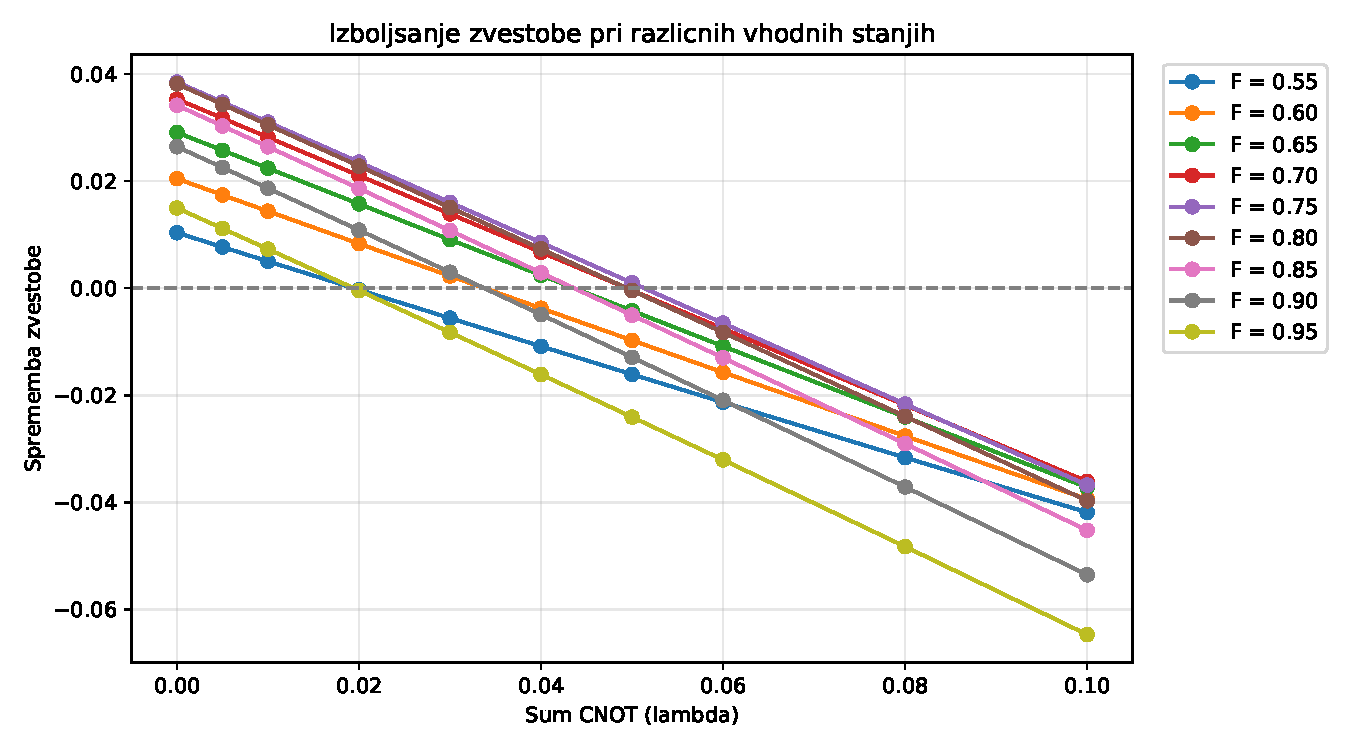
\includegraphics[width=0.94\textwidth]{izboljsanje_sum.pdf}
\caption{Sprememba zvestobe po enem krogu očiščevanja pri različnih vhodnih zvestobah in parametrih šuma CNOT. Rezultati natančne simulacije gostotnih matrik.}
\label{g24:fig:sprememba}
\end{figure}

Kot konkreten primer v tabeli~\ref{g24:tab:primer80} navajam vhodno zvestobo 0,80. Pri idealnih vratih je izboljšanje približno 3,815 odstotne točke. Pri $\lambda=0{,}04$ je izboljšanje le še 0,732 odstotne točke, pri $\lambda=0{,}05$ pa je izhodna zvestoba že manjša od vhodne.

\begin{table}[htbp]
\centering
\caption{Vpliv šuma na rezultate pri začetni zvestobi $F=0{,}80$.}
\label{g24:tab:primer80}
\begin{tabular}{rrrr}
\toprule
$\lambda$ & $F_{\mathrm{izhod}}$ & $P_{\mathrm{uspeh}}$ & Vhodnih parov na izhod \\
\midrule
0,000 & 0,838150 & 0,768889 & 2,6012 \\
0,010 & 0,830486 & 0,763538 & 2,6194 \\
0,020 & 0,822792 & 0,758241 & 2,6377 \\
0,030 & 0,815069 & 0,752998 & 2,6561 \\
0,040 & 0,807320 & 0,747808 & 2,6745 \\
0,050 & 0,799543 & 0,742672 & 2,6930 \\
0,100 & 0,760309 & 0,717800 & 2,7863 \\
\bottomrule
\end{tabular}
\end{table}

Slika~\ref{g24:fig:zvestoba80} prikazuje izhodno zvestobo pri začetni zvestobi $F=0{,}80$. Dokler je krivulja nad črtkano črto, očiščevanje izboljša zvestobo. Pri večjem šumu pade pod začetno vrednost.

\begin{figure}[htbp]
\centering
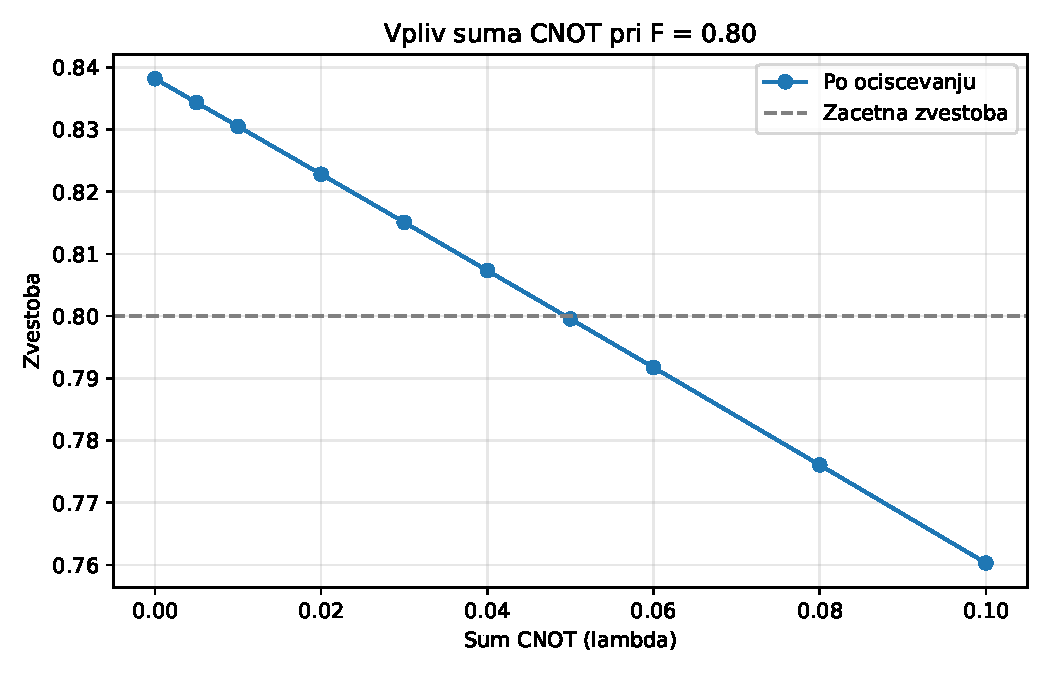
\includegraphics[width=0.83\textwidth]{zvestoba_sum.pdf}
\caption{Izhodna zvestoba po enem krogu BBPSSW pri začetni zvestobi $F=0{,}80$. Črtkana črta označuje začetno zvestobo.}
\label{g24:fig:zvestoba80}
\end{figure}

\subsection{Meja povečanja zvestobe}

Za natančnejšo določitev meje sem poleg vnaprej izbranih 90 kombinacij uporabil numerično iskanje ničle funkcije $\Delta F(\lambda)$. Rezultati so v tabeli~\ref{g24:tab:meje} in na sliki~\ref{g24:fig:meja}. Začetna zvestoba 0,75 ima med preverjenimi primeri največjo mejo $\lambda\approx0{,}051317$. Pri višjih in nižjih začetnih zvestobah je meja manjša.

Za uporabljeni model depolarizacijskega šuma lahko mejni parameter izračunamo tudi analitično. Iz pogoja $F_{\mathrm{izhod}}=F_{\mathrm{vhod}}$ dobimo

\begin{equation}
  \lambda_{\mathrm{meja}}(F)
  =1-\frac{3}{\sqrt{10-16(F-0{,}75)^2}}.
  \label{g24:eq:meja_analiticno}
\end{equation}

Formula je simetrična okoli $F=0{,}75$, ker nastopa kvadrat razlike $(F-0{,}75)^2$. Pri tej vrednosti je imenovalec največji, zato je največji tudi dovoljeni šum. Dobimo $\lambda_{\mathrm{meja}}(0{,}75)\approx0{,}051317$. Numerično izračunani pragovi se z analitičnimi vrednostmi ujemajo na šest decimalnih mest.

\begin{table}[htbp]
\centering
\caption{Izračunana meja depolarizacijskega parametra $\lambda$, kjer velja $F_{\mathrm{izhod}}=F_{\mathrm{vhod}}$.}
\label{g24:tab:meje}
\begin{tabular}{rrr}
\toprule
$F_{\mathrm{vhod}}$ & $\lambda_{\mathrm{meja}}$ & $P_{\mathrm{uspeh}}$ na meji \\
\midrule
0,55 & 0,0194193 & 0,576923 \\
0,60 & 0,0337651 & 0,601660 \\
0,65 & 0,0436349 & 0,630081 \\
0,70 & 0,0494136 & 0,662651 \\
0,75 & 0,0513167 & 0,700000 \\
0,80 & 0,0494136 & 0,742972 \\
0,85 & 0,0436349 & 0,792683 \\
0,90 & 0,0337651 & 0,850622 \\
0,95 & 0,0194193 & 0,918803 \\
\bottomrule
\end{tabular}
\end{table}

\begin{figure}[htbp]
\centering
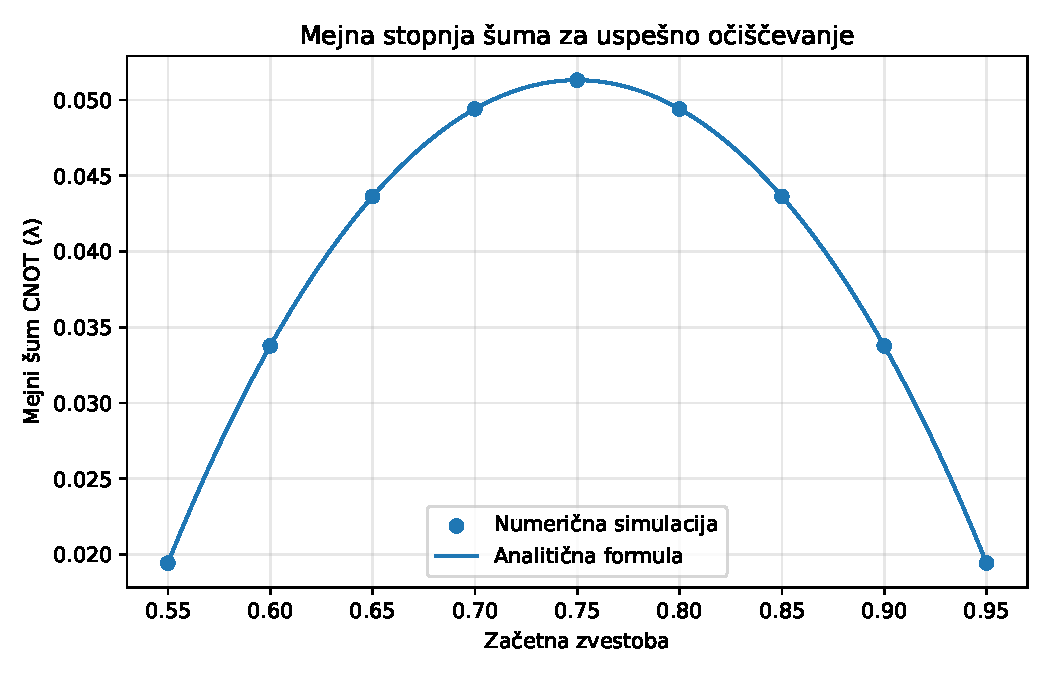
\includegraphics[width=0.83\textwidth]{pragi_suma.pdf}
\caption{Mejne vrednosti šuma CNOT, pri katerih se izhodna zvestoba izenači z vhodno. Točke predstavljajo rezultate numerične bisekcije, krivulja pa analitično formulo.}
\label{g24:fig:meja}
\end{figure}

\subsection{Verjetnost uspeha, poraba in zahtevnost vezja}

Že idealni protokol je verjetnosten: oba vhodna para uporabimo pri vsakem poskusu, vendar sprejmemo samo del izidov. Pri $F=0{,}80$ je verjetnost uspeha pri $\lambda=0$ približno 76,89~\%, pri $\lambda=0{,}10$ pa 71,78~\%. Hkrati se povprečna poraba vhodnih parov poveča z 2,60 na 2,79. Posamezne vrednosti so navedene v tabeli~\ref{g24:tab:primer80}.

Jedro protokola ima štiri kubite, dve vrati CNOT in dve meritvi. Pred transpilacijo je globina vezja 2, po transpilaciji za simulator \texttt{AerSimulator} s stopnjo optimizacije 1 pa prav tako 2. Število vrat CNOT se ne spremeni in ostane 2. Meritvi sta vključeni v globino, medtem ko priprava vhodnih mešanih stanj ni vključena v te strukturne metrike. Vpliv preslikave na konkretno topologijo fizičnega procesorja v tem preizkusu ni bil obravnavan.

\subsection{Statistična negotovost meritev}

Poleg natančne simulacije gostotnih matrik sem preveril še vpliv končnega števila meritev na oceno verjetnosti uspeha. Uporabil sem začetno zvestobo $F=0{,}80$ in šum $\lambda=0{,}05$, pri katerih je natančna verjetnost uspeha $P_{\mathrm{uspeh}}=0{,}742672$. Za vsako število meritev (1024, 4096 in 16384) sem izvedel 30 serij z različnimi naključnimi semeni.

V vsaki seriji sem preštel izida 00 in 11 ter njuno skupno število delil s številom meritev. Iz 30 ocen sem izračunal povprečje in vzorčni standardni odklon. Rezultate sem primerjal s teoretičnim standardnim odklonom

\begin{equation}
  \sigma_P = \sqrt{\frac{P_{\mathrm{uspeh}}(1-P_{\mathrm{uspeh}})}{N}},
  \label{g24:eq:odklon}
\end{equation}

kjer je $N$ število meritev. Rezultati so zbrani v tabeli~\ref{g24:tab:meritve}.

\begin{table}[htbp]
\centering
\caption{Primerjava izmerjene in teoretične statistične negotovosti pri $F=0{,}80$ in $\lambda=0{,}05$.}
\label{g24:tab:meritve}
\begin{tabular}{rrrr}
\toprule
$N$ & Povprečje $P$ & Odklon (sim.) & Odklon (teor.) \\
\midrule
1024  & 0,741732 & 0,016373 & 0,013661 \\
4096  & 0,742619 & 0,006744 & 0,006831 \\
16384 & 0,743052 & 0,003751 & 0,003415 \\
\bottomrule
\end{tabular}
\end{table}

\begin{figure}[htbp]
\centering
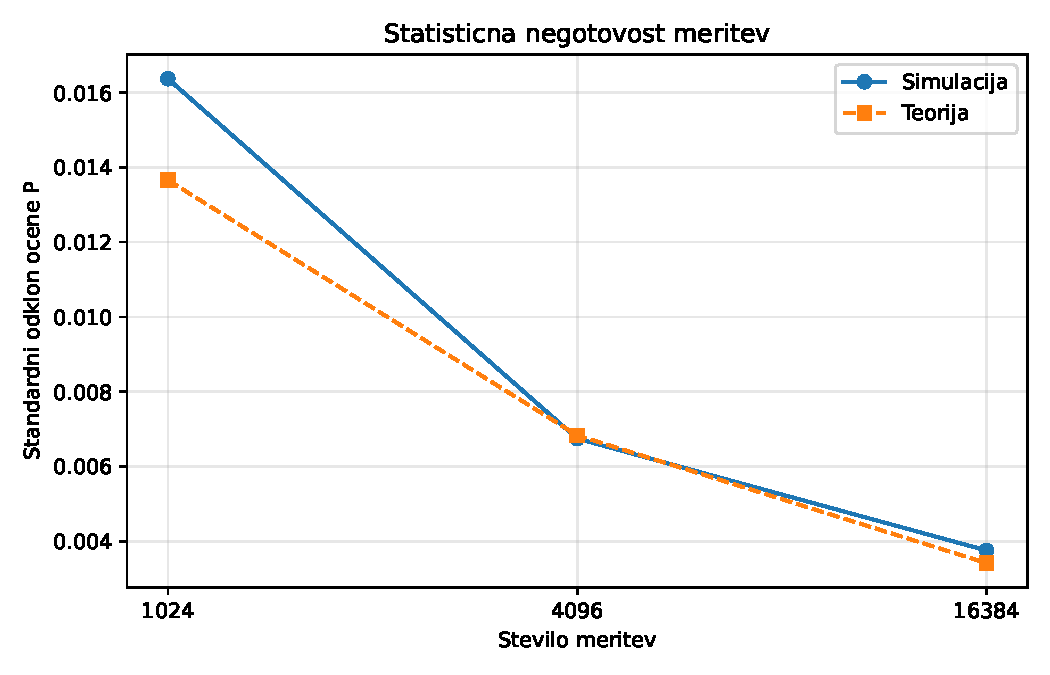
\includegraphics[width=0.83\textwidth]{odklon_meritev.pdf}
\caption{Standardni odklon ocene verjetnosti uspeha pri različnih številih meritev. Prikazana je primerjava 30 simuliranih serij s teoretičnim pričakovanjem.}
\label{g24:fig:meritve}
\end{figure}

Kot kaže slika~\ref{g24:fig:meritve}, se razpršenost ocen zmanjšuje z večanjem števila meritev. Pri 4096 meritvah se izmerjeni in teoretični standardni odklon skoraj ujemata. Manjša odstopanja so posledica ocenjevanja standardnega odklona iz 30 serij.

\section{Razprava}
\label{g24:sec:razprava}

Rezultati kažejo, da je izboljšanje zvestobe odvisno tako od vhodnega stanja kot od šuma na vratih CNOT. V idealnem primeru se je zvestoba pri vseh preverjenih Wernerjevih vhodnih stanjih povečala, kar je skladno z analitično rekurzijo BBPSSW. Ko sem dodal šum na CNOT, se je izboljšanje zmanjševalo. Za vsak obravnavani $F$ sem našel mejni parameter, nad katerim končna zvestoba ni več večja od začetne.

Oblika krivulje meje kaže, da imajo pri izbranem modelu vhodni pari z zvestobo okoli 0,75 največ rezerve za napake dodatnih vrat. Pri $F$ blizu 0,50 je idealni učinek očiščevanja razmeroma majhen, zato ga lahko že manjše napake odpravijo. Pri $F$ blizu 1 pa je par že skoraj idealen in je prostor za dodatno izboljšanje omejen. Šum tako v obeh primerih lažje prevlada nad koristjo očiščevanja.

Simetrija mejnih vrednosti ni samo lastnost narisanega grafa, ampak sledi tudi iz analitične enačbe~\eqref{g24:eq:meja_analiticno}. Tako imata na primer vhodni zvestobi $F=0{,}70$ in $F=0{,}80$ enak mejni parameter $\lambda\approx0{,}049414$. Ta rezultat velja za uporabljeni model dveh enakih Wernerjevih parov in depolarizacijskega šuma na obeh vratih CNOT. Pri drugačnem modelu napak takšne simetrije ne moremo samodejno pričakovati.

Meje iz tabele~\ref{g24:tab:meje} je treba razumeti kot \emph{prage povečanja zvestobe}. Ne pomenijo neposredno optimalne porabe virov ali najprimernejše strategije za kvantno komunikacijo. Na primer, na meji pri $F=0{,}80$ velja $F_{\mathrm{izhod}}=F_{\mathrm{vhod}}$, za sprejeti izhod pa porabimo v povprečju skoraj 2,69 vhodnega para. Zato je pri tem kriteriju očitno smiselneje uporabiti vhodni par brez dodatnega očiščevanja. Pri pozitivni, vendar majhni spremembi zvestobe bi bilo treba korist presoditi glede na namen uporabe.

\paragraph{Omejitve poskusa.}
Preveril sem samo en krog protokola, dve enaki Wernerjevi vhodni stanji in isti depolarizacijski kanal po obeh vratih CNOT. Merilne napake, napake priprave, izgube med prenosom parov, pomnilniška dekoherenca in koreliran šum niso vključeni. Šum izbranega depolarizacijskega kanala ni enak dejanskemu modelu vseh napak konkretnega kvantnega procesorja. Glavne rezultate sem izračunal neposredno iz gostotnih matrik, zato pri njih ni statistične negotovosti zaradi končnega števila meritev. V ločenem poskusu sem s končnim številom meritev ocenjeval verjetnost uspeha, ne pa izhodne zvestobe. Na fizičnem procesorju bi bilo treba iz meritev oceniti tudi zvestobo in upoštevati njeno statistično negotovost.

\subsection{Kaj ni delovalo}
\label{g24:sec:neuspehi}

Pri $F=0{,}80$ in parametru šuma $\lambda=0{,}05$ očiščevanje ni izboljšalo zvestobe vhodnega para. Izhodna zvestoba je znašala $0{,}799543$, čeprav je protokol sprejel približno 74,27\,\% poskusov. Pri tej stopnji šuma napake vrat CNOT izničijo izboljšanje, ki ga omogoča očiščevanje. Ta primer pokaže, da uspešna postselekcija še ne pomeni izboljšanja zvestobe.

\section{Zaključek}
\label{g24:sec:zakljucek}

Z lastno štirikubitno simulacijo sem preveril, kdaj en krog očiščevanja BBPSSW poveča zvestobo Wernerjevih Bellovih parov ob napakah vrat CNOT. Idealni rezultati so se ujemali z izvirno analitično formulo. Z depolarizacijskim šumom sem za devet začetnih zvestob določil meje, pri katerih izboljšanje izzveni. Pri $F=0{,}80$ znaša mejni parameter približno $0{,}049414$, največji med preverjenimi primeri pa približno $0{,}051317$ pri $F=0{,}75$.

Pokazalo se je, da uspešno očiščevanje v smislu sprejetja merilnih rezultatov še ne zagotavlja izboljšanja zvestobe. Poleg tega vsak uspešen izhod porabi več vhodnih parov. Delo bi bilo mogoče razširiti z merilnim šumom, realističnejšim šumnim modelom, več krogi očiščevanja ali ocenjevanjem zvestobe iz končnega števila meritev.

\section*{Doprinosi avtorjev}
Naloga je individualna. Žan Roštan je samostojno pripravil programsko okolje, zasnoval in izvedel simulacije idealnega in šumnega protokola ter izračunal mejne parametre in pripravil grafe. Odgovoren je tudi za analizo in interpretacijo rezultatov ter pripravo poročila in predstavitve.

\section*{Izjava o uporabi generativne umetne inteligence}
Pri delu sem uporabljal orodje ChatGPT (OpenAI) izključno kot podporno orodje pri iskanju in razumevanju strokovnih virov, preverjanju pravilnosti programske kode in razumevanju morebitnih napak ter oblikovanju, izboljšavi in jezikovnem urejanju besedila. Programsko okolje, programsko kodo, simulacije, izračune in analizo rezultatov sem pripravil oziroma izvedel samostojno. Simulacije sem izvajal lokalno v okolju Qiskit Aer. V poročilu so navedene uporabljene metode, parametri in datoteke, potrebne za ponovitev rezultatov.